% # COPYRIGHT:
%
% Copyright (C) 2011 Jeremiah Mahler <jmmahler@gmail.com>.
% Permission is granted to copy, distribute and/or modify this document
% under the terms of the GNU Free Documentation License, Version 1.3
% or any later version published by the Free Software Foundation;
% with no Invariant Sections, no Front-Cover Texts, and no Back-Cover Texts.
% A copy of the license is included in the file "fdl-1.3.txt".
%
\documentclass[12pt]{article}
%\usepackage{mslapa}
\usepackage{hyperref}
\usepackage{amsmath}
\usepackage{graphicx}
\usepackage{ulem}
\usepackage{vmargin}
\usepackage{tabularx}
\usepackage{sectsty}
\usepackage{pbox}
\usepackage{bigstrut}
\usepackage{enumerate}
\usepackage{parskip} % add spaces between paragraphs
\input kvmacros % Karnaugh Maps and Veitch charts
%\usepackage{cleveref}
\usepackage{verbatim}

\setpapersize{USletter}
\setmarginsrb{1.0in}{1.0in}{1.0in}{1.0in}{0in}{0.25in}{0in}{0.20in}

\sectionfont{\normalsize}
\subsectionfont{\normalsize}

% configure \bigstrut size
% This configures spacing above and below rows in a tabularx.
%\renewcommand{\bigstrutjot}{6pt}

\renewcommand{\bigstrutjot}{2.0\jot}

\setlength{\parindent}{0in}

\raggedright

\begin{document}

% {{{ Cover Page
\centerline{\bf EECE 144}
\centerline{\bf Fall 2011}
\centerline{\bf}
\centerline{\bf Lab Report \#9}
\centerline{\bf Section 4}
\centerline{\bf 11/2/2011}
% signature area
\begin{center}
\begin{tabularx}{\textwidth}[b]{X l l}
Submitted by: Jeremiah Mahler & & \\
Signature & Printed Name & Date \\
\hline
\multicolumn{1}{|X|}{} & \multicolumn{1}{|l|}{\bigstrut \bf Jeremiah Mahler} & \multicolumn{1}{|l|}{\bf Nov 02, 2011} \\
\hline
\multicolumn{1}{|X|}{} & \multicolumn{1}{|l|}{\bigstrut \bf Marvanee Johnson} & \multicolumn{1}{|l|}{\bf Nov 02, 2011} \\
\hline
\end{tabularx}
\end{center}
% }}}

% {{{ Description/Objectives
\section{Description/Objectives}

The objective of this lab is to introduce Verilog \cite{VERILOG}
and GTKWave \cite{GTKWAVE} by construction a function to implement
a two-bit adder.  The function is defined by Table \ref{tbl:tt}.

\begin{table}[hbp]
\begin{center}
\begin{tabular}{lr}
\begin{tabular}[t]{r|cccc|ccc}
 & $A_1$ & $A_0$ & $B_1$ & $B_0$ & $C$ & $S_1$ & $S_0$ \\
\hline
0  & 0 & 0 & 0 & 0 & 0 & 0 & 0\\
1  & 0 & 0 & 0 & 1 & 0 & 0 & 1\\
2  & 0 & 0 & 1 & 0 & 0 & 1 & 0\\
3  & 0 & 0 & 1 & 1 & 0 & 1 & 1\\
4  & 0 & 1 & 0 & 0 & 0 & 0 & 1\\
5  & 0 & 1 & 0 & 1 & 0 & 1 & 0\\
6  & 0 & 1 & 1 & 0 & 0 & 1 & 1\\
7  & 0 & 1 & 1 & 1 & 1 & 0 & 0\\
8  & 1 & 0 & 0 & 0 & 0 & 1 & 0\\
9  & 1 & 0 & 0 & 1 & 0 & 1 & 1\\
10 & 1 & 0 & 1 & 0 & 1 & 0 & 0\\
11 & 1 & 0 & 1 & 1 & 1 & 0 & 1\\
12 & 1 & 1 & 0 & 0 & 0 & 1 & 1\\
13 & 1 & 1 & 0 & 1 & 1 & 0 & 0\\
14 & 1 & 1 & 1 & 0 & 1 & 0 & 1\\
15 & 1 & 1 & 1 & 1 & 1 & 1 & 0\\
\end{tabular}
\end{tabular}
\end{center}
\caption{Truth table of the two bit adder.  The two bit number \{ $A_1$, $A_0$ \}
is added to the two bit number \{ $B_1$, $B_0$ \} resulting in the two bit number
\{ $S_1$, $S_0$ \} with the carry bit $C$.}
\label{tbl:tt}
\end{table}

% }}}

% {{{ Procedure
\section{Procedure}
\label{sec:procedure}

To construct the two bit adder in Verilog requires several steps.
First, three functions corresponding to each output (Table \ref{tbl:tt})
must be found and minimized using Karnaugh Maps.
Then these functions must be defined in the Verilog format.
Then the Verilog file must be compiled and run and its outputs
verified against the desired outputs from the truth table.
Additionally, GTKWave is used to graphically visualize all the
state changes over time.

The first function to be found is for the output $C$.
The Karnaugh Map for this function is shown in Figure \ref{fig:kmc}.
Grouping the 1s together results in SOP Equation \ref{eq:c}.

\begin{figure}
\begin{center}
\karnaughmap{4}{$C(a, b, c, d)$:}{abcd}{0000000100110111}{}
\end{center}
\caption{Karnaugh map of function $C$.
The variables $a$, $b$, $c$ and $d$ correspond to
$A_1$, $A_0$, $B_1$, $B_0$ in Table \ref{tbl:tt}.}
\label{fig:kmc}
\end{figure}

\begin{equation}
C = A_1 B_1 + A_0 B_1 B_0 + A_1 A_0 B_0 \label{eq:c}
\end{equation}

Next the output of the function $S_1$ is found.
Its Karnaugh Map is shown in Figure \ref{fig:kms1}
Grouping the 1s together results in SOP Equation \ref{eq:s1}.

\begin{figure}
\begin{center}
\karnaughmap{4}{$S_1(a, b, c, d)$:}{abcd}{0011011011001001}{}
\end{center}
\caption{Karnaugh map of function $S_1$.
The variables $a$, $b$, $c$ and $d$ correspond to
$A_1$, $A_0$, $B_1$, $B_0$ in Table \ref{tbl:tt}.}
\label{fig:kms1}
\end{figure}

\begin{equation}
S_1 = A_1 B_1' B_0'
	+ A_1 A_0' B_1'
	+ A_1 A_0 B_1 B_0
	+ A_1' A_0 B_1' B_0
	+ A_1' A_0' B_1
	+ A_1' B_1 B_0' \label{eq:s1}
\end{equation}

Finally the output of the function $S_0$ is found.
Its Karnaugh Map is shown in Figure \ref{fig:kms0}
Grouping the 1s together results in SOP Equation \ref{eq:s0sop}.
And this equation can be simplified using XOR as shown in Equation \ref{eq:s0}.

\begin{figure}
\begin{center}
\karnaughmap{4}{$S_0(a, b, c, d)$:}{abcd}{0101101001011010}{}
\end{center}
\caption{Karnaugh map of function $S_1$.
The variables $a$, $b$, $c$ and $d$ correspond to
$A_1$, $A_0$, $B_1$, $B_0$ in Table \ref{tbl:tt}.}
\label{fig:kms0}
\end{figure}

\begin{align}
S_0 &= A_0 B_0' + A_0' B_0 \label{eq:s0sop} \\
	&= A_0 \oplus B_0 \label{eq:s0}
\end{align}

Now that the three functions corresponding to the three outputs have
been found this can be programmed in Verilog.
In Verilog there is more than one way to construct a module.
Here we are using \emph{data flow modeling} with operators and
primitives.
This form is very verbose and specifies each step explicitly
(see Appendix \ref{sec:source} for the full source code).
In contrast, if \emph{data flow modeling} was used, it would
describe the operation at a higher (behavioral) level by using
\verb+if+, \verb+case+, loops and other operations.

Once the source code is entered it must be compiled.
The example below shows how this was done using Icarus Verilog \cite{VERILOG}
under Linux.

\begin{verbatim}
shell$ ls
adder.v
shell$ iverilog adder.v
shell$ ls
adder.v  a.out
\end{verbatim}

The file 'a.out' is the executable produced during compilation.
Next the executable is run.

\begin{verbatim}
shell$ ./a.out 
VCD info: dumpfile gtkwave-02.vcd opened for output.
a1 a0 b1 b0 | c s1 s0
---------------------
0  0  0  0  | 0  0  0
0  0  0  1  | 0  0  1
0  0  1  0  | 0  1  0
0  0  1  1  | 0  1  1
0  1  0  0  | 0  0  1
0  1  0  1  | 0  1  0
0  1  1  0  | 0  1  1
0  1  1  1  | 1  0  0
1  0  0  0  | 0  1  0
1  0  0  1  | 0  1  1
1  0  1  0  | 1  0  0
1  0  1  1  | 1  0  1
1  1  0  0  | 0  1  1
1  1  0  1  | 1  0  0
1  1  1  0  | 1  0  1
1  1  1  1  | 1  1  0
shell$ ls
adder.v  a.out  gtkwave-02.vcd
\end{verbatim}

In this case the \verb+$display+ statements were arranged so that
a truth table was output.
This can be used to verify that the outputs agree with the
truth table of the desired values (Table \ref{tbl:tt}).
Also notice that the file \verb+gtkwave-02.vcd+ has been created.
This file can be used with GTKWave to produce a display of the wave
forms over time.

\begin{verbatim}
shell$ gtkwave gtkwave-02.vcd
\end{verbatim}

% }}}

% {{{ Observations
\section{Observations}

The output values produced by Verilog agreed with those in the
truth table of desired values.
And GTKWave correctly displayed the bit values over time
as shown in Figure \ref{fig:wave}

\begin{figure}
\center
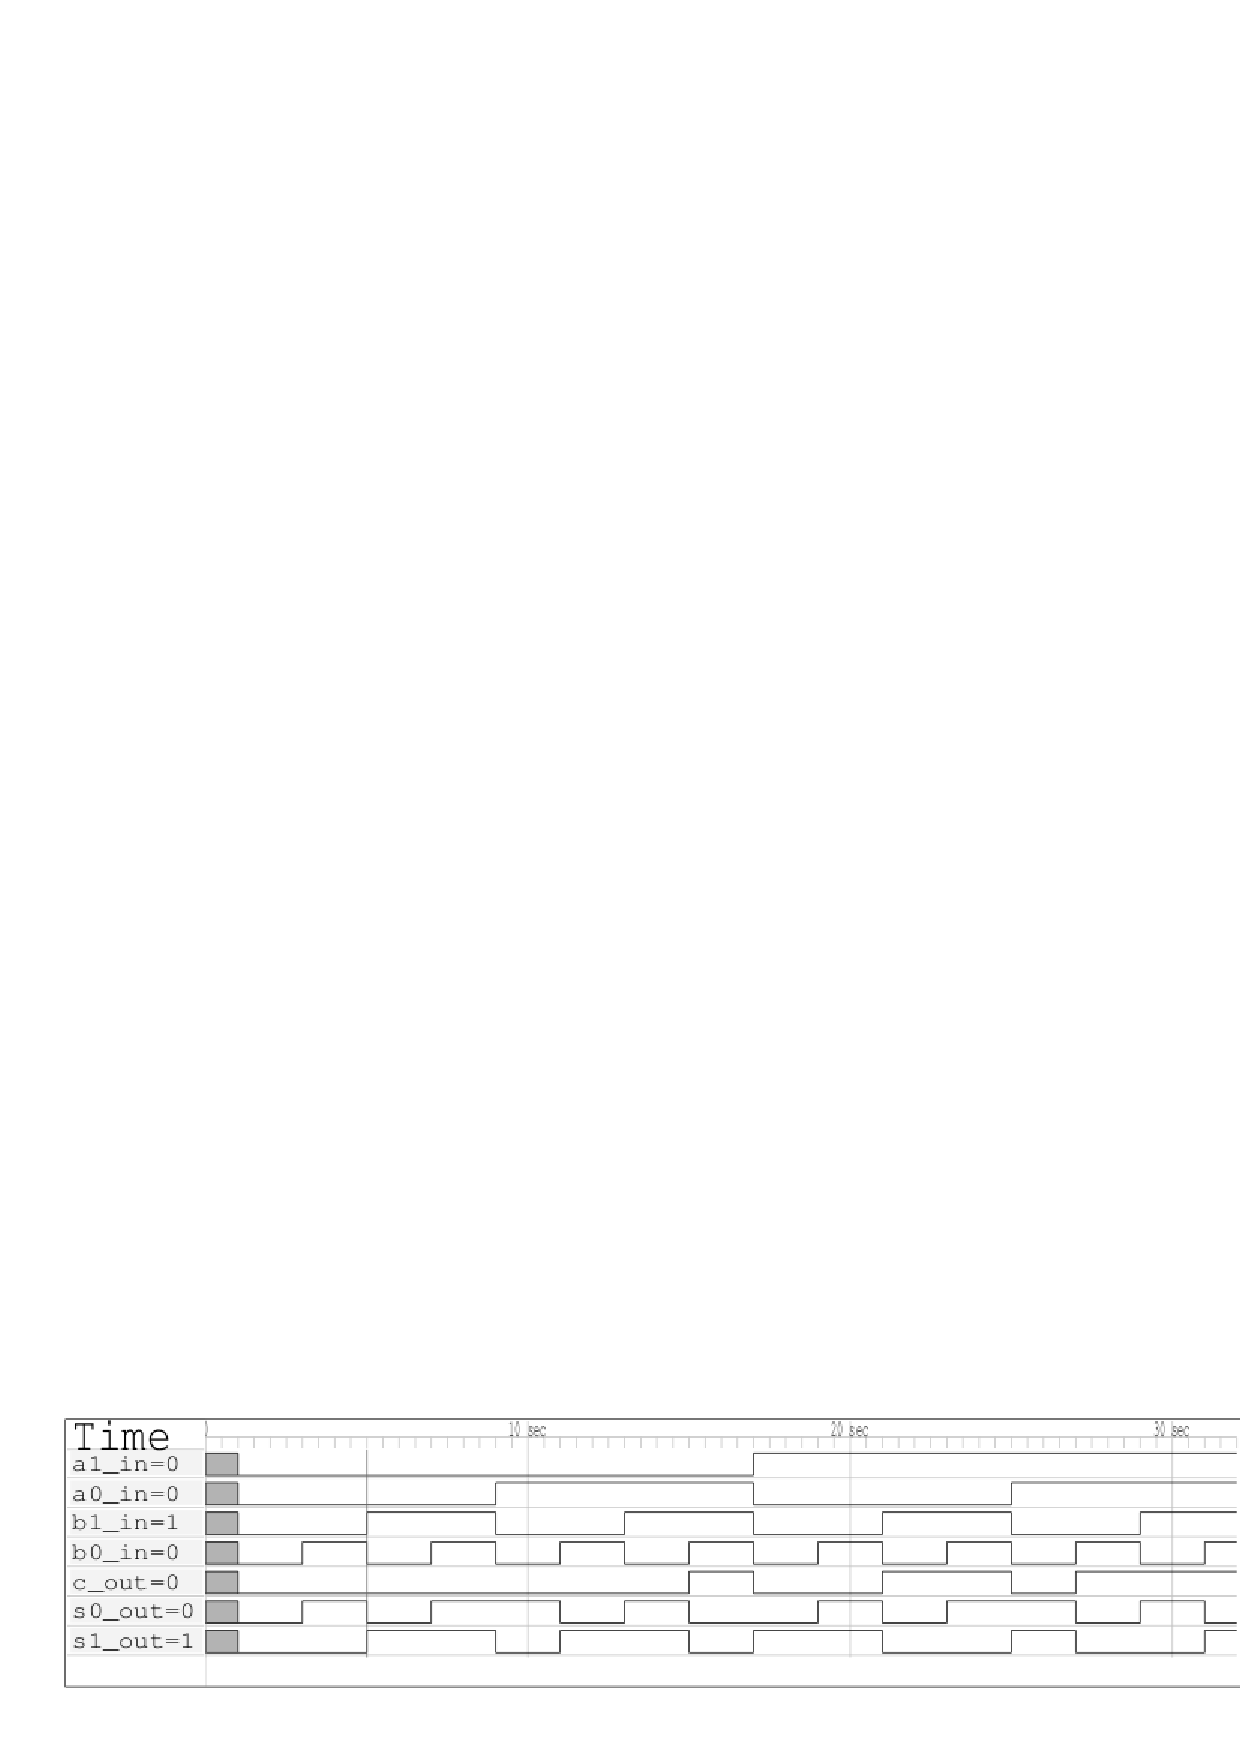
\includegraphics[scale=0.7]{verilog/gtkwave-output}
\caption{Output of GTKWave.
The left column shows the variable names corresponding to their wave form.
The names have been changed slightly as compared to the definition in Table \ref{tbl:tt}.
For example a0\_in is $A_0$, b1\_in is $B_1$, s1\_out is $S_1$, and so on.
In general output variables have \_out appended and input variables have \_in appended.
}
\label{fig:wave}
\end{figure}

Verilog, just like every other programming language, has its own
unique quirks and caveats that can trick even seasoned programmers.
For example, Verilog uses the concept of 'modules' and they
seem similar to functions in C.
But their behavior is quite different.
Conceptually using a module is like placing a gate on to a circuit,
it will operate without needing to be called.
Also Verilog is very specific about times.
For example, if a \verb+$display$+ statement does not have a delay
from a previous data assignment it may display the data before the
assignment.
See the source code in Appendix \ref{sec:source} for more details.

% }}}

% {{{ Conclusion
\section{Conclusion}

This lab was a success in introducing Verilog and GTKWave for analysis
of digital circuits and creation of a two bit adder.

% }}}

\renewcommand*{\refname}{\vspace{-8mm}}
\section{References}
%%\bibliographystyle{plain}
%%\bibliographystyle{mslapa}
\bibliographystyle{ieeetr}
\bibliography{../references}

\appendix

\clearpage
\section{Verilog Source}
\label{sec:source}

{\footnotesize
\verbatiminput{verilog/adder.v}
}

\end{document}

% vim:foldmethod=marker
